\documentclass[11pt]{article}
\usepackage[T1]{fontenc} % para que pueda partir palabras con acentos
\usepackage[utf8]{inputenc}
\usepackage{rotating}
\usepackage{graphicx}
\usepackage[spanish]{babel} % Ojo que esto cambia el nombre de las secciones
\usepackage{times,url}
\usepackage{amsmath}
\usepackage{mathrsfs}
\usepackage{amsfonts}
\usepackage{amssymb}
% \usepackage{hyphen}
% \hyphenation{car-dú-me-nes dis-con-ti-nui-da-des}
\usepackage{fullpage}

\usepackage[a4paper,bottom=2.7cm,top=2.7cm,left=2.5cm,right=2.5cm]{geometry}
\usepackage{fancyhdr} % Esto cambiará la ubicación de los numeritos de las páginas
\usepackage{grffile} % Para tipear nombres de archivo con espacios
%\usepackage{esvect} % Para poner flechas de vector más copadas
\usepackage{array} % Paquete que mejora la funcionalidad de array

% Carga de paquetes extra
\usepackage{color}
\usepackage{colortbl}
\usepackage{tocloft}
\usepackage{setspace}
\usepackage{titlesec}
\usepackage{fix-cm}
\usepackage{natbib}
\setcitestyle{square}
\usepackage{multirow}
\usepackage{bigstrut}

\usepackage{wrapfig}
\usepackage{enumitem}
\usepackage{appendix}

\usepackage{mdframed}
\usepackage{listings}
\definecolor{light-gray}{gray}{0.95}

% Se carga la hoja de estilo
\usepackage{RT_estilo} 
\usepackage{fancyvrb}

% Fracciones bonitas
\usepackage{nicefrac}

\usepackage{listings}
\usepackage{xcolor}
% Definir un color personalizado 'cremita'
\definecolor{cremita}{RGB}{255,253,208}

\lstset{
  backgroundcolor=\color{cremita}, % Usar el color 'cremita' como fondo
    frame=single, % añade un recuadro simple alrededor del código
    framerule=0pt, % grosor del borde del recuadro
    framesep=3pt, % espacio entre el recuadro y el contenido
    rulecolor=\color{gray}, % color del recuadro
    xleftmargin=\parindent, % margen izquierdo
    xrightmargin=0px, % margen derecho
}


\usepackage{hyperref}
\hypersetup{
    colorlinks=false, % Establece colorlinks en falso para desactivar los enlaces de color
    pdfborder={0 0 0}, % Establece el borde del PDF a 0 para eliminar el recuadro
}

\PassOptionsToPackage{hyphens}{url}\usepackage{hyperref}

\usepackage{pdflscape}

%\renewcommand{\topfraction}{0.85}
%\renewcommand{\bottomfraction}{0.85}
%\renewcommand{\textfraction}{0.1}
%\renewcommand{\floatpagefraction}{0.75}
%\setcounter{topnumber}{4}
%\setcounter{bottomnumber}{3}
%\setcounter{totalnumber}{6}

\usepackage{float}
\usepackage{placeins}

% Aumentar la proporción de flotantes permitidos por página hasta la sección específica
\newcommand{\relaxFloats}{
    \renewcommand{\topfraction}{0.85}
    \renewcommand{\bottomfraction}{0.85}
    \renewcommand{\textfraction}{0.1}
    \renewcommand{\floatpagefraction}{0.75}
    \setcounter{topnumber}{4}
    \setcounter{bottomnumber}{3}
    \setcounter{totalnumber}{6}
}

% Restaurar a los valores por defecto a partir de una sección específica
\newcommand{\restoreFloats}{
    \renewcommand{\topfraction}{0.7}
    \renewcommand{\bottomfraction}{0.3}
    \renewcommand{\textfraction}{0.2}
    \renewcommand{\floatpagefraction}{0.5}
    \setcounter{topnumber}{2}
    \setcounter{bottomnumber}{1}
    \setcounter{totalnumber}{3}
}

% =====================================================================================================
% =====================================================================================================
%
% DOCUMENTO PROPIAMENTE DICHO
%
% =====================================================================================================
% =====================================================================================================

\begin{document}

% =====================================================================================================
% =====================================================================================================
% PORTADA
% =====================================================================================================
% =====================================================================================================
\thispagestyle{empty}

%	==============================================================
%	Caja Superior
%	==============================================================

	\noindent
	\begin{minipage}[c][50mm][c]{1.0\linewidth} 
		\begin{center}
			\Large{\textbf{\underline{PROYECTO}: Monitoreo acústico de niveles de ruido submarino y telemetría satelital para detección de eventos acústicos intensos en aguas de la Plataforma Continental Argentina}}\\
%			\Large{\textbf{}}\\
			\vspace{2mm}		
			\textbf{Dirección del proyecto:}\hspace{2pc}\textit{Igor Prario}\\
			\textbf{Co-Dirección del proyecto:}\hspace{2pc}\textit{Patricio Bos}\\
		\end{center}
	\end{minipage}
	\vspace{1mm}

%	============================================================== 
% 	Caja Central
%	==============================================================

	\noindent
	\begin{minipage}[c][70mm][c]{1.0\linewidth} 
		{\hrule\hrule}
% 		\vspace{1mm}
% 		\textcolor{blue}{\hrule\hrule}
 		\vspace{5mm}
		\begin{flushleft}
			\huge{Rutinas de configuración y adquisición para interfaz de audio Behringer}
		\end{flushleft}
		\vspace{8mm}
		\begin{flushright}
			\Large{Patricio Bos}\\
		\end{flushright}
		\vspace{2mm}
		{\hrule\hrule}
% 		\vspace{1mm}
% 		\textcolor{blue}{\hrule\hrule}
	\end{minipage}
	\vspace{-5mm}

	\noindent
	\begin{minipage}[c][30mm][c]{1.0\linewidth} 		
		\begin{flushright}
			\Large{División Acústica Submarina\\
				Informe Técnico AS 3/25\\
				Marzo 2025}\\
		\end{flushright}
	\end{minipage}
	\vspace{5mm}
	
%	==============================================================	
% 	Caja inferior
%	==============================================================

	\noindent
	\begin{minipage}[c][60mm][c]{1.0\linewidth} 
% 		\begin{table}[h]
			\begin{minipage}[c]{0.39\linewidth}
				\centering
				
\includegraphics[width=0.55\textwidth]{graficos/ESCUDO.jpg}
			\end{minipage}
			\hspace*{1pc}
			\begin{minipage}[c]{0.60\linewidth}
				\begin{center}
					\Huge{\textbf{DIIV}}\\
					\Large{DIRECCIÓN DE\\ 
					INVESTIGACIÓN DE LA ARMADA}\\
				\end{center}
			\end{minipage}			
			\begin{minipage}[c]{1.0\linewidth}
				\hfill\vspace{4mm}
			\end{minipage}
			\begin{minipage}[c]{0.40\linewidth}
				\centering
				
\includegraphics[width=1.0\textwidth]{graficos/LOGO_UNIDEF_SOLO.jpg}
			\end{minipage}
			\hspace*{1pc}
			\begin{minipage}[c]{0.60\linewidth}
				\begin{center}
					\Huge{\textbf{UNIDEF}}\\					
					\Large{UNIDAD EJECUTORA DE\\
					INVESTIGACIÓN Y DESARROLLO\\
					ESTRATÉGICOS PARA LA DEFENSA}\\
					CONICET/MINDEF\\
				\end{center}
			\end{minipage}
% 		\end{table}
	\end{minipage}		

\clearpage

% =====================================================================================================
% =====================================================================================================
% PÁGINA DE RESUMEN EN CASTELLANO Y EN INGLÉS
% =====================================================================================================
% =====================================================================================================

\begin{center}
	\large{\textbf{\textcolor{black}{Rutinas de configuración y adquisición para anemómetro Gill WindSonic.}}}\\
	\vspace{1pc}
	\textbf{Marcos Remotti y Patricio Bos}
\end{center}

\bigskip
	\begin{center}
		\textcolor{black}{RESUMEN}	
	\end{center}
	\begin*
		\indent
		\textit{El presente informe técnico documenta el diseño e implementación de un módulo de software para configurar y controlar un anemómetro Gill WindSonic. Este instrumento forma parte del equipamiento de la Estación Autónoma Marítima para el Monitoreo de Ruido Ambiente (EAMMRA), desarrollado por la División Acústica Submarina de la Dirección de Investigación de la Armada (DIIV). El software desarrollado permite la adquisición y registro de datos de viento de manera automática o manual, mediante un archivo de argumentos configurables por el usuario.
Este trabajo es parte del Proyecto ``Monitoreo acústico de niveles de ruido submarino y telemetría satelital para detección de eventos acústicos intensos en aguas de la Plataforma Continental Argentina'', del programa PIDDEF del Ministerio de Defensa, vinculado al Proyecto ``Localización e identificación de fuentes de ruido'' de la Armada Argentina, llevado a cabo en la División Acústica Submarina de la Dirección de Investigación de la Armada (DIIV) y la Unidad Ejecutora de Investigación y Desarrollo Estratégicos para la Defensa (UNIDEF), dependiente de CONICET/MinDef.}
	\end*

\bigskip
	\begin{center}
		\textcolor{black}{ABSTRACT}
	\end{center}
	\begin*
		\indent
		\textit{This technical report documents the design and implementation of a software module for configuring and controlling a Gill WindSonic anemometer. This instrument is part of the equipment of the Autonomous Maritime Station for Ambient Noise Monitoring (EAMMRA), developed by the Underwater Sound Division of the Argentinian Navy Research Office (DIIV). The developed software allows for the acquisition and recording of wind data automatically or manually, through a user-configurable argument file.
This work is part of the Project ``Acoustic monitoring of underwater noise levels and satellite telemetry for detecting intense acoustic events in waters of the Argentine Continental Shelf'', from the PIDDEF program of the Ministry of Defense, linked to the Project ``Localization and identification of noise sources'' of the Argentine Navy, carried out in the Underwater Sound Division of the Argentinian Navy Research Office (DIIV) and the Strategic Research and Development Unit for Defense (UNIDEF), dependent on CONICET/MinDef.} 
	\end*

\clearpage


% =====================================================================================================
% =====================================================================================================
% PÁGINA DESCRIPTIVA DE PERTENENCIA A PROYECTO DEL TRABAJO
% =====================================================================================================
% =====================================================================================================



\vspace*{170pt}

\begin{center}
	\begin{tabular}[c]{c}
% 		\arrayrulecolor{red}
		\hline\hline
		\\
		\Large{Este trabajo es parte del Proyecto}\vspace{2mm}\\
		\Large{``Monitoreo acústico de niveles de ruido submarino y telemetría satelital}\vspace{2mm}\\ 
		\Large{para detección de eventos acústicos intensos en aguas de la }\vspace{2mm}\\ 
		\Large{Plataforma Continental Argentina'',}\vspace{2mm}\\
		\Large{del programa PIDDEF del Ministerio de Defensa,}\vspace{2mm}\\ 
		\Large{vinculado al Proyecto ``Localización e identificación de fuentes de ruido''}\vspace{2mm}\\ 
		\Large{de la Armada Argentina,}\vspace{2mm}\\ 
		\Large{que se lleva a cabo en la División Acústica Submarina}\vspace{2mm}\\ 
		\Large{del Departamento Investigación de la Armada (DIIV) y}\vspace{2mm}\\ 
		\Large{la Unidad Ejecutora de Investigación y Desarrollo Estratégicos}\vspace{2mm}\\
		\Large{para la Defensa (UNIDEF), dependiente de CONICET/MinDef.}\vspace{8mm}\\
		\hline\hline
	\end{tabular}
\end{center}

\clearpage

% =====================================================================================================
% =====================================================================================================
% PÁGINA DE AGRADECIMIENTOS
% =====================================================================================================
% =====================================================================================================
% La configuración está optimizada para fotos de 3cm de ancho (armónicamente).  
%

%
\begin{center}
	\Large\textbf{{\textcolor{black}{AGRADECIMIENTOS}}}
\end{center}Los autores desean expresar su agradecimiento a:

\vspace{2pc}

\begin{minipage}[c]{0.2\linewidth}
	\frame{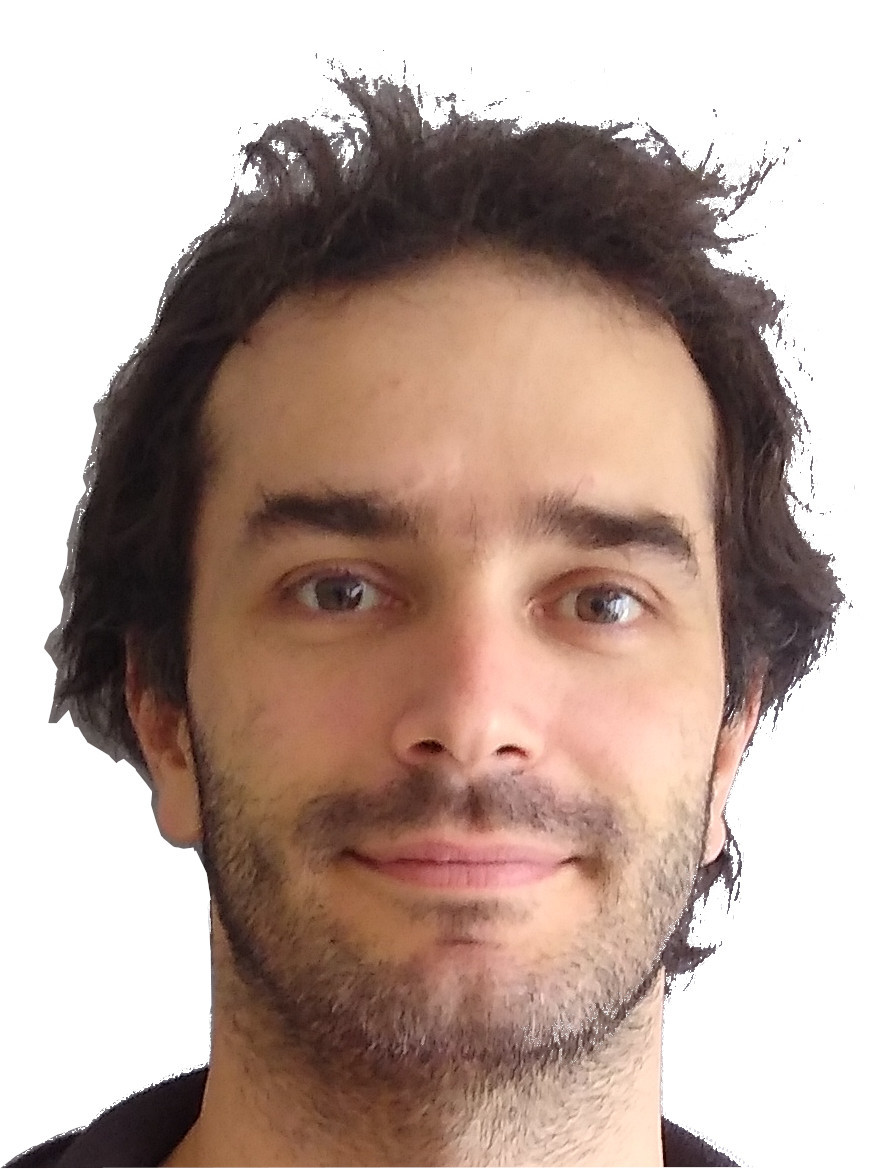
\includegraphics[width=.7\textwidth]{graficos/Foto_carnet_AGCV_Rojo.jpg}}
\end{minipage}
\hfill
\begin{minipage}[c]{0.7\linewidth}
	Ing. Rui Marques Rojo, investigador RPIDFA que forma parte del equipo de trabajo del Departamento de Propagación Acústica de la Dirección de Investigación de la Armada, por el montaje y puesta a punto de la plataforma Gitea con servicios para el desarrollo de código, que fuera extensamente utilizada en la realización del trabajo que aquí se documenta.  Asimismo, se deja constancia de sus valiosas sugerencias para la implementación de código en lenguaje Python.
\end{minipage}%\vfill

\vspace{2pc}
\clearpage


% =====================================================================================================
% =====================================================================================================
% ÍNDICE
% =====================================================================================================
% =====================================================================================================


\tableofcontents
\clearpage


% =====================================================================================================
% =====================================================================================================
% GLOSARIO DE SIGLAS
% =====================================================================================================
% =====================================================================================================


\begin{center}
	\Large\textbf{{\textcolor{black}{GLOSARIO DE SIGLAS}}}
\end{center}
\begin{tabular}{l p{12cm}}
%	AH		&Amper hora.\\
	API		&Application Program Interface.\\		
	ARA		&Armada Argentina.\\
	ASCII	&American Standard Code for Information Interchange.\\
	AWG		&American Wire Gauge.\\
	CD		&Continuous Delivery.\\
	CI		&Continuous Integration.\\
	CSV		&Comma Separated Values.\\	
	DDR		&Double Data Rate.\\
	EAMMRA	&Estación Autónoma Marítima para el Monitoreo de Ruido Ambiente.\\
	ETX		&End of TeXt.\\
	GB		&Giga Byte.\\	
	GNU		&Gnu is Not Unix.\\
	IDE		&Integrated Development Environment.\\
	LTS		&Long Term Support.\\
	LAN		&Local Area Network.\\
	MIL-DTL	&Military Detail Specification.\\
    NMEA	&National Marine Electronics Association.\\	
	PCM		&Pulse Code Modulation.\\	
	PEP		&Python Enhancement Proposal.\\
	RIFF	&Resource Interchange File Format.\\
	SSH		&Secure SHell.\\	
	URL		&Uniform Resource Locators.\\
	VPN		&Virtual Private Network.\\
	WAV		&WAVeform audio file.\\
	YAML	&YAML Ain't Markup Language.\\
\end{tabular}

\clearpage


% =====================================================================================================
% =====================================================================================================
% LISTA DE FIGURAS
% =====================================================================================================
% =====================================================================================================

\begin{center}
\listoffigures
\end{center}
\clearpage

% =====================================================================================================
% =====================================================================================================
% LISTA DE TABLAS
% =====================================================================================================
% =====================================================================================================
%
%\begin{center}
%\listoftables
%\end{center}
%\clearpage

% =====================================================================================================
% =====================================================================================================
% CUERPO DEL INFORME
% =====================================================================================================
% =====================================================================================================

\section{INTRODUCCIÓN}

%\subsection{Objetivo}

El objetivo de este informe técnico es documentar el diseño e implementación de un módulo de software para configurar y controlar una placa de audio Behringer UMC204HD.  Este dispositivo forma parte del equipamiento e instrumental de la Estación Autónoma Marítima para el Monitoreo de Ruido Ambiente (EAMMRA) que se desarrolla en la División Acústica Submarina de la Dirección de Investigación de la Armada (DIIV). 

La estación EAMMRA es una boya de superficie de diseño específico para la medición de Ruido Ambiente submarino cuya concepción, diseño y fabricación se encuentran documentados en respectivos informes técnicos \citep{EAMMRA_ingConceptual}, \citep{EAMMRA_diseno} y \citep{EAMMRA_subsistemas}.  

El control de la estación en general, y la interacción con la placa en particular, se realizan con una computadora de grado industrial Kaise KBOX-S J6412. Esta computadora pertenece a la categoría de \textit{fanless embedded systems}, que son sistemas de misión específica sin partes móviles y es especialmente adecuada para aplicaciones de funcionamiento autónomo.  Cuenta con un procesador Intel Celeron J6412 de cuatro núcleos y memoria DDR4 de 16 GB \citep{kaise}, lo que le otorga al sistema una razonable capacidad de cómputo para el bajo consumo de energía que requiere la aplicación. En la figura \ref{fig:kaise} se muestra una vista frontal y trasera de la computadora y se pueden observar las interfaces y conectores disponibles.
 
\begin{figure}[htpb]
    \centering
    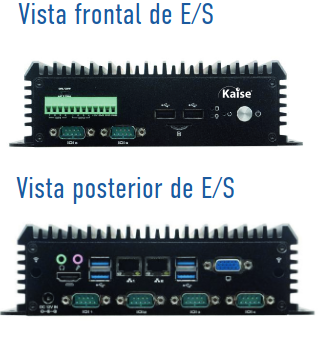
\includegraphics[width=.44\textwidth]{graficos/kaise.png}
    \caption{Vista frontal y trasera de la computadora Kaise KBOX-S J6412.}
    \label{fig:kaise}
\end{figure}


La computadora de EAMMRA corre un sistema operativo de propósitos generales, Ubuntu Server 22.04 LTS. Ubuntu Server es una distribución libre y gratuita de GNU/Linux que no requiere la compra de licencias para su uso. Este sistema operativo es reconocido por su estabilidad y seguridad, atributos esenciales para aplicaciones críticas en sistemas desatendidos como EAMMRA. Por diseño, Ubuntu Server permite una extensa personalización, con la posibilidad de realizar una instalación con los mínimos componentes necesarios, lo que permite optimizar el rendimiento general del sistema.

El módulo de software para configurar y controlar la placa de audio se implementa en Python, un lenguaje de programación interpretado y multiparadigma de alto nivel que viene integrado por defecto en las distribuciones de Ubuntu. En particular, para este módulo se utiliza Python3 que es la versión del lenguaje recomendada para proyectos nuevos, que no requieren retrocompatibilidad con componentes previos que hayan sido desarrollados en Python2.


\subsection{Herramientas de desarrollo}

Las herramientas de desarrollo de software que se utilizaron para la implementación del módulo de configuración y control permiten mejorar la calidad del código. Se entiende como código de calidad, aquel que hace lo que se supone que debe hacer, no contienen defectos ni problemas y es fácil de extender con nuevas características.

Las guías de estilo en general se utilizan para definir una forma consistente de escribir código. Si bien el estilo de codificación puede parecer una cuestión de forma, que no afecta el funcionamiento lógico del código, algunas decisiones de estilo pueden evitar errores lógicos frecuentes. Las guías definen convenciones que ayudan a mantener el código fácil de leer, mantener y extender.

Se emplearon herramientas específicas para lenguaje Python, que tienen gran difusión y aceptación en la comunidad de desarrolladores conocidas como \textit{linters}.  Estas herramientas permiten analizar el código y verificar el cumplimiento de un conjunto de reglas de mejores prácticas y buscan problemas, tanto de no conformidad con un estilo como errores de lógica.  Los defectos de lógica que se buscan son errores de código, código con resultados potencialmente no deseado y patrones de código peligroso. El uso de estas herramientas mejora la legibilidad, la mantenibilidad y la escalabilidad y hace que el código sea menos propenso a errores.   


\subsubsection{Guías de estilo para código Python - PEP-8 y PEP-257}

Para la escritura del código Python del módulo de configuración y control se adopta la guía de estilo \textit{Python Enhancement Proposal} 8 (PEP-8). Su objetivo principal es mejorar la legibilidad y coherencia del código Python y tiene amplia aceptación dentro de la comunidad de desarrolladores de este lenguaje. La guía fue escrita en 2001 por Guido van Rossum, Barry Warsaw y Nick Coghlan, basándose en las mejores prácticas existentes y las recomendaciones de la comunidad \citep{pep8}. Esta guía fomenta buenas prácticas y técnicas que pueden ayudar a evitar errores comunes.

La guía cubre varios aspectos de la codificación, que incluyen:

\begin{itemize}
	\item Formato del código: indentación, uso de espacios en blanco, longitud de las líneas, etc.
	\item Convenciones de nomenclatura: cómo nombrar variables, funciones, clases, módulos, etc.
	\item Principios de codificación: recomendaciones sobre cómo escribir expresiones y declaraciones de manera clara.
	\item Comentarios: cuándo y cómo usar comentarios para mejorar la legibilidad del código.
\end{itemize}

Asimismo, se utiliza la convención \textit{Python Enhancement Proposal} 257, (PEP-257).  Esta convención define el formato y estilo para la documentación, también llamada \textit{Python's docstrings} que aplica a módulos, clases, funciones y métodos \citep{pep257}.  Adicionalmente, si los \textit{docstring} se escriben en forma consistente, existen herramientas capaces de generar documentación directamente del código.  Esto permite mantener más fácilmente la documentación actualizada dentro del mismo código.

Existen herramientas de desarrollo como pycodestyle y pydocstyle que verifican el estilo y ayudan a asegurar que el código cumpla con las convenciones de PEP-8 y PEP-257, respectivamente.  Estas herramientas pertenecen a la categoría de linters de estilo y en algunos casos vienen integrados dentro de otros linters como Flake8 o Pylama.

\subsubsection{Style guide enforcement - Flake8}

Flake8 es una herramienta que permite imponer y hacer cumplir las directivas de la guía de estilo PEP-8 y pertenece a la familia de programas tipo \textit{lint} que trabajan analizando el código fuente para verificar el cumplimiento de un conjunto definido de reglas. Esta herramienta puede señalar errores de programación, \textit{bugs}, errores de estilo y construcciones sospechosas. Es altamente configurable, y permite a los desarrolladores ajustar las reglas y la severidad de las advertencias según las necesidades específicas de su proyecto \citep{flake8}.

Para instalar flake8 para la versión por defecto de Python:

\begin{lstlisting}[language=bash]
python -m pip install flake8
\end{lstlisting}

Para utilizar flake8, se deben ejecutar los siguientes comando desde una terminal interactiva:

\begin{lstlisting}[language=bash]
flake8 path/to/code/to/check.py
# or
flake8 path/to/code/
\end{lstlisting}

%\clearpage

A su vez, se puede seleccionar una regla específica para ejecutar o ignorar:

\begin{lstlisting}[language={python}]
flake8 --select E123,W503 path/to/code/
# or
flake8 --extend-ignore E203,W234 path/to/code/
\end{lstlisting}

El listado completo de códigos de error y su significado puede encontrarse en el sitio web oficial de la herramienta, \url{http://flake8.pycqa.org/en/latest/user/error-codes.html}.

\subsubsection{Analizador estático - Pylint}
Pylint es una herramienta de análisis estático de código para Python que busca errores de programación, ayuda a hacer cumplir un estándar de codificación y busca ``malos olores'' en el código (\textit{code smells}). Utiliza diferentes técnicas para analizar el código fuente y puede identificar problemas o patrones de codificación problemáticos que podrían llevar a errores o a un código difícil de mantener o leer \citep{pylint}. 

Las características principales de Pylint incluyen:

\begin{itemize}
    \item Chequeo de errores: puede detectar errores que podrían hacer que el código falle en tiempo de ejecución, como llamadas a funciones no definidas, uso de variables antes de su definición, etc.
    \item Estándares de codificación: Pylint puede asegurar de que el código siga un estándar de codificación particular, como PEP-8.
    \item Refactorización de código: sugiere lugares donde el código podría ser refactorizado para mejorar la legibilidad o la eficiencia.
    \item Detección de código duplicado: puede identificar bloques de código duplicados que podrían ser simplificados o extraídos en una función común.
    \item Chequeo de tipos: aunque Python es un lenguaje dinámicamente tipado, Pylint puede realizar algunas comprobaciones de tipos para identificar posibles problemas.
\end{itemize}

Para instalar pylint para la versión por defecto de Python:

\begin{lstlisting}[language=bash]
python -m pip install pylint
\end{lstlisting}

Para utilizar pylint, se debe ejecutar el siguiente comando:

\begin{lstlisting}[language=bash]
pylint [options] modules_or_packages
\end{lstlisting}

%\begingroup %inexplicablemente esto hace que la url fittee bien 
%\sloppy
%
%\endgroup

Pylint agrega un prefijo a cada una de las áreas problemáticas con una R, C, W, E o F, que significan:

\begin{itemize}
    \item \textbf{R}efactorizar por una violación de la métrica de ``buena práctica''.
    \item \textbf{C}onvención por violación del estándar de codificación.
    \item \textbf{W}arning (Advertencia) por problemas estilísticos o problemas de programación menores.
    \item \textbf{E}rror por problemas importantes de programación (es decir, muy probablemente un bug).
    \item \textbf{F}atal por errores que impidieron el procesamiento adicional.
\end{itemize}

La lista completa de mensajes y su significado puede encontrarse en el sitio web oficial de la herramienta, donde se encuentran agrupados por categoría o área problemática.  La url es: \small{\url{https://pylint.pycqa.org/en/latest/user_guide/messages/messages_overview.html}}.

\subsubsection{Formato automático - Black}

Black es una herramienta de formateo de código para Python conocida por su enfoque en la simplicidad y la uniformidad. A menudo se le llama ``el formateador de código sin compromisos'' debido a su filosofía de tener una sola forma estandarizada y automatizada de formatear el código Python. Esto contrasta con otras herramientas de formateo que pueden permitir una mayor configuración o variaciones en el estilo de codificación \citep{black}.

Algunas características clave de Black incluyen:

\begin{itemize}
    \item Automatización: Black reformatea todo el archivo de código con solo un comando, sin necesidad de ajustes manuales.
    \item Consistencia: aplica un estilo consistente en todos los proyectos de Python al seguir un conjunto de reglas predefinido, lo que ayuda a mejorar la legibilidad y reducir el tiempo dedicado a discutir sobre estilos de codificación en revisiones de código.
    \item Integración fácil: puede integrarse fácilmente con editores de texto y entornos de desarrollo integrados (IDEs), así como con sistemas de integración continua/entrega continua (CI/CD).
    \item Seguridad: está diseñado para realizar cambios en el código que no afecten su comportamiento, lo que lo hace seguro para usar en proyectos grandes y complejos.
\end{itemize}

Al tener el código un formato unificado entre los distintos desarrolladores, las revisiones de código, especialmente bajo control de versiones, se pueden hacer más rápidamente debido a que los \textit{diffs }entre versiones son lo más pequeños posible.  Black es un formateador de código PEP-8 compatible.

Para instalar Black, se debe ejecutar el siguiente comando en una terminal:

\begin{lstlisting}[language=bash]
python pip install black
\end{lstlisting}

Para utilizar Black, se debe ejecutar el siguiente comando:

\begin{lstlisting}[language=bash]
black modules_or_packages
\end{lstlisting}

\subsubsection{Entorno de Desarrollo Integrado - Visual Studio Code}

Visual Studio Code, disponible en \url{https://code.visualstudio.com/}, es un editor de código fuente de código abierto que soporta múltiples lenguajes de programación. Destaca por su flexibilidad y capacidad de personalización. Permite integrar extensiones que amplían sus funcionalidades. Entre sus características se encuentran el soporte para depuración integrada, control de versiones con Git y herramientas de autocompletado. También ofrece una interfaz de usuario intuitiva y un sistema de gestión de proyectos eficiente. VSCode es compatible con Windows, macOS y GNU/Linux.

Existen múltiples extensiones disponibles para Python. Entre las más destacadas se encuentran el \textit{plugin} \texttt{Python}, que proporciona soporte para depuración, ejecución de código, y autocompletado de código Python, y \texttt{Pylance}, que ofrece características adicionales como análisis estático de código y autocompletado inteligente.

La extensión Remote - SSH de Visual Studio Code permite utilizar cualquier máquina remota con un servidor SSH como entorno de desarrollo. Esto facilita el desarrollo y la resolución de problemas en una amplia variedad de situaciones. Mediante esta extensión, es posible desarrollar en el mismo sistema operativo al que se desplegará el software o emplear hardware más grande, rápido o especializado que el de la máquina local.

Una de las ventajas de esta extensión es la capacidad de cambiar rápidamente entre diferentes entornos de desarrollo remotos, lo que permite realizar actualizaciones de manera segura sin riesgo de afectar la máquina local. Además, proporciona acceso a un entorno de desarrollo ya existente desde varias máquinas o ubicaciones, lo que aumenta la flexibilidad del proceso de desarrollo.

Esta extensión resulta útil también para depurar aplicaciones que se ejecutan en otros lugares. No es necesario tener el código fuente en la máquina local para aprovechar estas ventajas, ya que la extensión ejecuta comandos y otras extensiones directamente en la máquina remota. Es posible abrir cualquier carpeta en la máquina remota y trabajar con ella de la misma forma que si estuviera en la máquina local.

\subsubsection{Pytest}

Pytest \citep{pytest} es un marco de pruebas o \textit{framework} para Python que facilita la creación, ejecución y gestión de pruebas automatizadas. Su diseño simple y flexible lo convierte en una herramienta popular tanto para desarrolladores novatos como para expertos. A través de una sintaxis intuitiva, pytest permite escribir pruebas concisas y efectivas, y ofrece potentes herramientas para la depuración de errores, la introspección de aserciones y la ejecución de pruebas en múltiples configuraciones. Es utilizado principalmente para pruebas unitarias, aunque también puede aplicarse a pruebas de integración y funcionales. pytest sigue un enfoque basado en convenciones, lo que significa que por defecto, descubre y ejecuta las pruebas sin necesidad de una configuración extensa.

Entre las características más destacadas de pytest se incluyen su sistema de \textit{fixtures}, que permite preparar datos y recursos reutilizables para las pruebas, y su potente mecanismo de aserciones, que ofrece introspección detallada de los errores durante los fallos de prueba. Además, pytest soporta pruebas parametrizadas, la ejecución de pruebas en paralelo mediante \textit{plugins}, y una fácil integración con herramientas de cobertura de código y análisis estático. Los resultados de las pruebas se presentan de forma clara y legible, y permiten que los desarrolladores comprendan rápidamente los problemas detectados. También es compatible con otras bibliotecas de pruebas como \texttt{unittest} y \texttt{nose}, lo que facilita la transición entre diferentes marcos de pruebas.

En cuanto a los requerimientos, pytest necesita Python 3.8 o superior para su funcionamiento, y puede instalarse fácilmente utilizando el administrador de paquetes \texttt{pip}. Para instalarlo, basta con ejecutar el siguiente comando: 
\begin{lstlisting}[language=bash]
pip install -U pytest
\end{lstlisting}

Una vez instalado, pytest se ejecuta desde la línea de comandos con el comando \texttt{pytest}, lo que hará que busque y ejecute todas las pruebas definidas en los archivos que sigan la convención de nombres \texttt{test\_*.py} o \texttt{*\_test.py}. Además, \texttt{pytest} permite la configuración avanzada mediante archivos de configuración y opciones de línea de comandos, lo que otorga una gran flexibilidad en proyectos de gran escala. La documentación oficial está disponible en \citep{pytest_documentation}.

\clearpage
\section{INTERFAZ DE AUDIO BEHRINGER UMC204HD}

La Behringer UMC204HD es una interfaz de audio USB que ofrece una conversión de señal precisa y confiable, \citep{behringerUMC204HD}. Se utiliza en la grabación y reproducción de señales de audio analógicas y digitales. Es adecuada para la adquisición de señales de hidrófonos en aplicaciones científicas como EAMMRA. En la figura \ref{fig:behringer} se puede observar una vista frontal y trasera de la interfaz.

\vspace{10px}
\begin{figure}[ht]
    \centering
    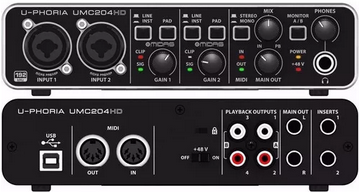
\includegraphics[width=.5\textwidth]{graficos/behringer.png}
    \caption[]{Vista frontal y trasera de la interface de audio Behringer UMC204HD.}
    \label{fig:behringer}
\end{figure}

La UMC204HD tiene dos entradas XLR/TRS combo para micrófonos o instrumentos. También cuenta con dos salidas balanceadas TRS 1/4” para una señal limpia. La interfaz soporta dos canales de entrada y salida simultáneos. Cada canal tiene control de ganancia independiente. Incluye salidas de auriculares con control de volumen y un monitor de mezcla directa para la monitorización sin latencia.

La interfaz tiene una resolución de 24 bits y soporta hasta 192 kHz. La relación señal/ruido supera los 100 dB, lo que reduce el ruido en la señal. Estos valores permiten una captura precisa de señales, como las de hidrófonos. La interfaz es compatible con varias plataformas de software, lo que la hace versátil.

Con Python y PyAudio, se puede controlar la interfaz para la adquisición de datos en tiempo real. PyAudio permite configurar la tasa de muestreo, los canales y otros parámetros. Esto facilita la integración de la interfaz en sistemas de adquisición y análisis de señales.

La interfaz de audio cuenta con múltiples conectores de tipo \emph{jack} para facilitar la conexión de micrófonos, instrumentos y sistemas de monitoreo. A continuación se detallan los principales tipos de conectores presentes en el panel frontal y trasero de la unidad:

\subsection*{Entradas de audio}

\begin{itemize}
    \item \textbf{Entradas combo XLR/TRS}: La unidad dispone de dos entradas combinadas (canales 1 y 2) que aceptan conectores XLR balanceados (para micrófonos) y jacks TRS de 6,35\,mm (1/4'') para señales de línea o instrumentos. Estas entradas se encuentran en el panel frontal y permiten selección de ganancia, alimentación phantom \mbox{+48\,V} y atenuación según el tipo de señal.
\end{itemize}

\subsection*{Salidas de audio}

\begin{itemize}
    \item \textbf{Salidas balanceadas TRS}: En el panel trasero se encuentran dos salidas principales (L y R) mediante jacks TRS de 6,35\,mm, que proporcionan señal balanceada para conexión a monitores de estudio o mezcladores.
    
    \item \textbf{Salidas RCA}: Adicionalmente, la unidad dispone de un par de salidas RCA no balanceadas (Line Out 1/2), útiles para conexión a sistemas domésticos o grabadoras externas.
    
    \item \textbf{Salida de auriculares}: En el panel frontal se encuentra un conector jack estéreo de 6,35\,mm para monitoreo con auriculares. Incluye control de volumen independiente y mezcla entre señal directa y reproducción desde el host.
\end{itemize}

Todos los conectores están montados en el chasis metálico de la interfaz, con fijación robusta para evitar fallos mecánicos durante el uso intensivo en laooratorio o en campo.



	
\clearpage
\section{DISEÑO E IMPLEMENTACIÓN }

\subsection{Descripción general del módulo}

El módulo \texttt{BehringerHandler} fue desarrollado en Python con el objetivo de controlar una interfaz de audio USB marca Behringer de forma programática. Permite su inicialización, apertura de flujos de entrada, grabación asincrónica y gestión completa de recursos. Está pensado para ser utilizado en sistemas de adquisición acústica en tiempo real, y su diseño modular facilita su integración en arquitecturas mayores, como estaciones de monitoreo o sistemas embebidos.

El funcionamiento interno del módulo se apoya en varias bibliotecas estándar y externas. Utiliza \texttt{pyaudio} para el acceso de bajo nivel al hardware de audio, \texttt{wave} para la escritura de los datos capturados en formato WAV, \texttt{threading} para realizar la grabación en paralelo al hilo principal y \texttt{queue} para sincronizar los datos entre procesos. Además, se emplean \texttt{logging} para la trazabilidad de eventos, \texttt{datetime} para la generación de nombres de archivo basados en marca temporal y \texttt{os} para la gestión del entorno de ejecución y rutas de archivo. Esta combinación de módulos permite una operación robusta, escalable y fácilmente depurable.

La biblioteca \texttt{logging} de Python se utiliza para generar registros estructurados durante la ejecución del código, y permite monitorear el estado del sistema, detectar errores y realizar trazabilidad de eventos. En el módulo \texttt{BehringerHandler}, se implementa un sistema de log dual que escribe tanto en consola como en un archivo de texto (\texttt{behringer\_handler.log}). Este sistema utiliza formatos personalizados con marcas de tiempo y niveles de severidad (INFO, WARNING, ERROR), lo que facilita el diagnóstico en tiempo real y la revisión posterior del funcionamiento del sistema. La inclusión de \texttt{logging} mejora la mantenibilidad y confiabilidad del software, especialmente en entornos donde no hay interacción directa con el usuario.

La biblioteca \texttt{PyAudio} proporciona una interfaz en Python para interactuar con PortAudio, una biblioteca de código abierto para la captura y reproducción de audio en tiempo real. Este paquete permite abrir flujos de entrada o salida de audio con parámetros configurables como tasa de muestreo, formato, número de canales y tamaño de buffer. En el caso de \texttt{BehringerHandler}, \texttt{PyAudio} es utilizado para detectar dispositivos de audio disponibles, abrir un flujo de entrada en formato \texttt{paInt24} y capturar señales a alta resolución (192 kHz, 2 canales). Gracias a su capacidad para operar en modo no bloqueante mediante callbacks, \texttt{PyAudio} permite implementar grabaciones asincrónicas eficientes, fundamentales para aplicaciones de adquisición continua o en tiempo real.

La biblioteca estándar \texttt{wave} de Python permite la manipulación de archivos de audio en formato WAV (RIFF). Proporciona una interfaz sencilla para la escritura y lectura de audio en formato PCM (Pulse Code Modulation), y permite definir parámetros como la cantidad de canales, la tasa de muestreo y la resolución en bits. En el módulo \texttt{BehringerHandler}, \texttt{wave} se utiliza para almacenar las grabaciones capturadas por el stream de PyAudio en archivos de alta calidad de 24 bits. La escritura se realiza en tiempo real desde un hilo separado, para asegurar la integridad de los datos y su disponibilidad inmediata en disco para posteriores análisis.

La biblioteca \texttt{threading} proporciona soporte para la ejecución concurrente de código mediante la creación y gestión de hilos de ejecución. En \texttt{BehringerHandler}, se utiliza para realizar la escritura de audio en disco de forma asincrónica, separando la captura en tiempo real del procesamiento de los datos. Esto permite que el flujo principal de adquisición no se vea interrumpido por operaciones de entrada/salida, lo que mejora el rendimiento y evita pérdidas de datos. El uso de \texttt{threading} resulta esencial para garantizar grabaciones continuas y confiables, especialmente en sistemas que requieren alta tasa de muestreo o baja latencia.

La biblioteca \texttt{queue} proporciona una estructura de datos segura para comunicación entre hilos en entornos multithreading. En el módulo \texttt{BehringerHandler}, se utiliza una instancia de \texttt{Queue} para almacenar de forma temporal los bloques de audio recibidos por el callback del stream de PyAudio. Esta cola permite desacoplar la adquisición de datos (en tiempo real) de la escritura en disco, evitando pérdidas o bloqueos por operaciones lentas de entrada/salida. El uso de \texttt{queue} garantiza una sincronización segura y eficiente entre el hilo de captura y el hilo de grabación.

La biblioteca estándar \texttt{datetime} permite manipular fechas y horas de manera precisa y flexible. En el módulo  \texttt{BehringerHandler}, se utiliza para generar marcas de tiempo en el momento de iniciar una grabación, lo que permite construir nombres de archivo únicos con el formato \texttt{YYYYMMDD\_HHMMSS}. Esta práctica facilita la organización de las grabaciones, evita sobreescrituras accidentales y proporciona una trazabilidad temporal inmediata. El uso de \texttt{datetime} también permite registrar eventos en los logs con exactitud temporal.

La biblioteca estándar \texttt{os} proporciona funciones para interactuar con el sistema operativo de forma portable. En el módulo \texttt{BehringerHandler}, se utiliza para obtener la ruta absoluta del script en ejecución, crear subdirectorios (como \texttt{recordings} para guardar archivos de audio) y construir rutas de forma segura e independiente del sistema operativo.  El uso de \texttt{os} es esencial para garantizar la correcta gestión de archivos y configuraciones en distintos entornos de ejecución.


\subsection{Dependencias y gestión del entorno}

La lista completa de dependencias necesarias para ejecutar el módulo \texttt{BehringerHandler} se encuentra documentada en el archivo \texttt{requirements.txt}. Este archivo fue generado utilizando el comando \texttt{pip freeze > requirements.txt} desde un entorno virtual de Python configurado específicamente para este proyecto. La utilización de entornos virtuales permite aislar las versiones de los paquetes, asegurando la reproducibilidad del entorno de ejecución.

Para reconstruir el entorno en una nueva máquina o entorno limpio, se recomienda crear un entorno virtual (por ejemplo, mediante \texttt{python -m venv venv}) y luego instalar todas las dependencias mediante el comando \texttt{pip install -r requirements.txt}. Esto garantiza que las versiones exactas utilizadas durante el desarrollo serán replicadas, y permite reducir los  errores por incompatibilidades entre bibliotecas.

A continuación, se presenta la lista de dependencias incluidas en \texttt{requirements.txt}:

\begin{verbatim}
Package         Version
--------------- -----------
astroid         3.3.9
black           25.1.0
click           8.1.8
contourpy       1.3.1
cycler          0.12.1
dill            0.3.9
flake8          7.2.0
fonttools       4.56.0
iniconfig       2.1.0
isort           6.0.1
kiwisolver      1.4.8
matplotlib      3.10.1
mccabe          0.7.0
mypy-extensions 1.0.0
numpy           2.2.3
packaging       24.2
pathspec        0.12.1
pillow          11.1.0
pip             25.0.1
platformdirs    4.3.7
pluggy          1.5.0
PyAudio         0.2.14
pycodestyle     2.13.0
pyflakes        3.3.2
pylint          3.3.6
pyparsing       3.2.1
pytest          8.3.5
python-dateutil 2.9.0.post0
schedule        1.2.2
six             1.17.0
tomlkit         0.13.2
\end{verbatim}


\subsection{Arquitectura del módulo}

El diseño del módulo \texttt{BehringerHandler} está centrado en encapsular toda la funcionalidad de adquisición de audio a través de una interfaz USB Behringer, utilizando una arquitectura modular y extensible. La clase actúa como fachada para todas las operaciones, ofreciendo una interfaz clara basada en un ciclo de vida típico: inicialización, grabación y liberación de recursos.

Este ciclo se articula mediante un conjunto de métodos públicos que definen el flujo de uso:

\begin{enumerate}
    \item \texttt{init()} inicializa la interfaz PyAudio y detecta automáticamente el dispositivo Behringer conectado por USB.
    \item \texttt{record(duration)} lanza una grabación asincrónica por el tiempo especificado. Internamente, abre el stream de entrada (\texttt{open()}), inicia un hilo de escritura en disco (\texttt{\_write\_audio()}) y activa un callback (\texttt{\_callback()}) que llena una cola de datos.
    \item \texttt{stop\_recording()} sincroniza el final de la grabación, deteniendo el hilo y limpiando los buffers.
    \item \texttt{deinit()} libera todos los recursos y deja el módulo en estado reutilizable.
\end{enumerate}

Desde el punto de vista del usuario, el uso del módulo sigue una secuencia lógica simple:

\begin{verbatim}
from behringer_handler import BehringerHandler

handler = BehringerHandler()
handler.init()
handler.record(duration=10)  # graba 10 segundos de audio
handler.stop_recording()
handler.deinit()
\end{verbatim}

Durante la ejecución, los datos son adquiridos por el stream de PyAudio y colocados en una cola mediante el callback. En paralelo, un hilo escribe esos datos en un archivo WAV. Todos los eventos relevantes —como el inicio o cierre del stream, errores o advertencias— se registran mediante el sistema de \texttt{logging}, tanto en consola como en un archivo de log.

Este diseño permite desacoplar la adquisición en tiempo real del almacenamiento en disco, reduciendo riesgos de pérdida de datos y manteniendo la modularidad del sistema. Además, garantiza una interfaz coherente con otros módulos de adquisición definidos dentro del sistema EAMRRA.

\begin{figure}[htpb]
    \centering
    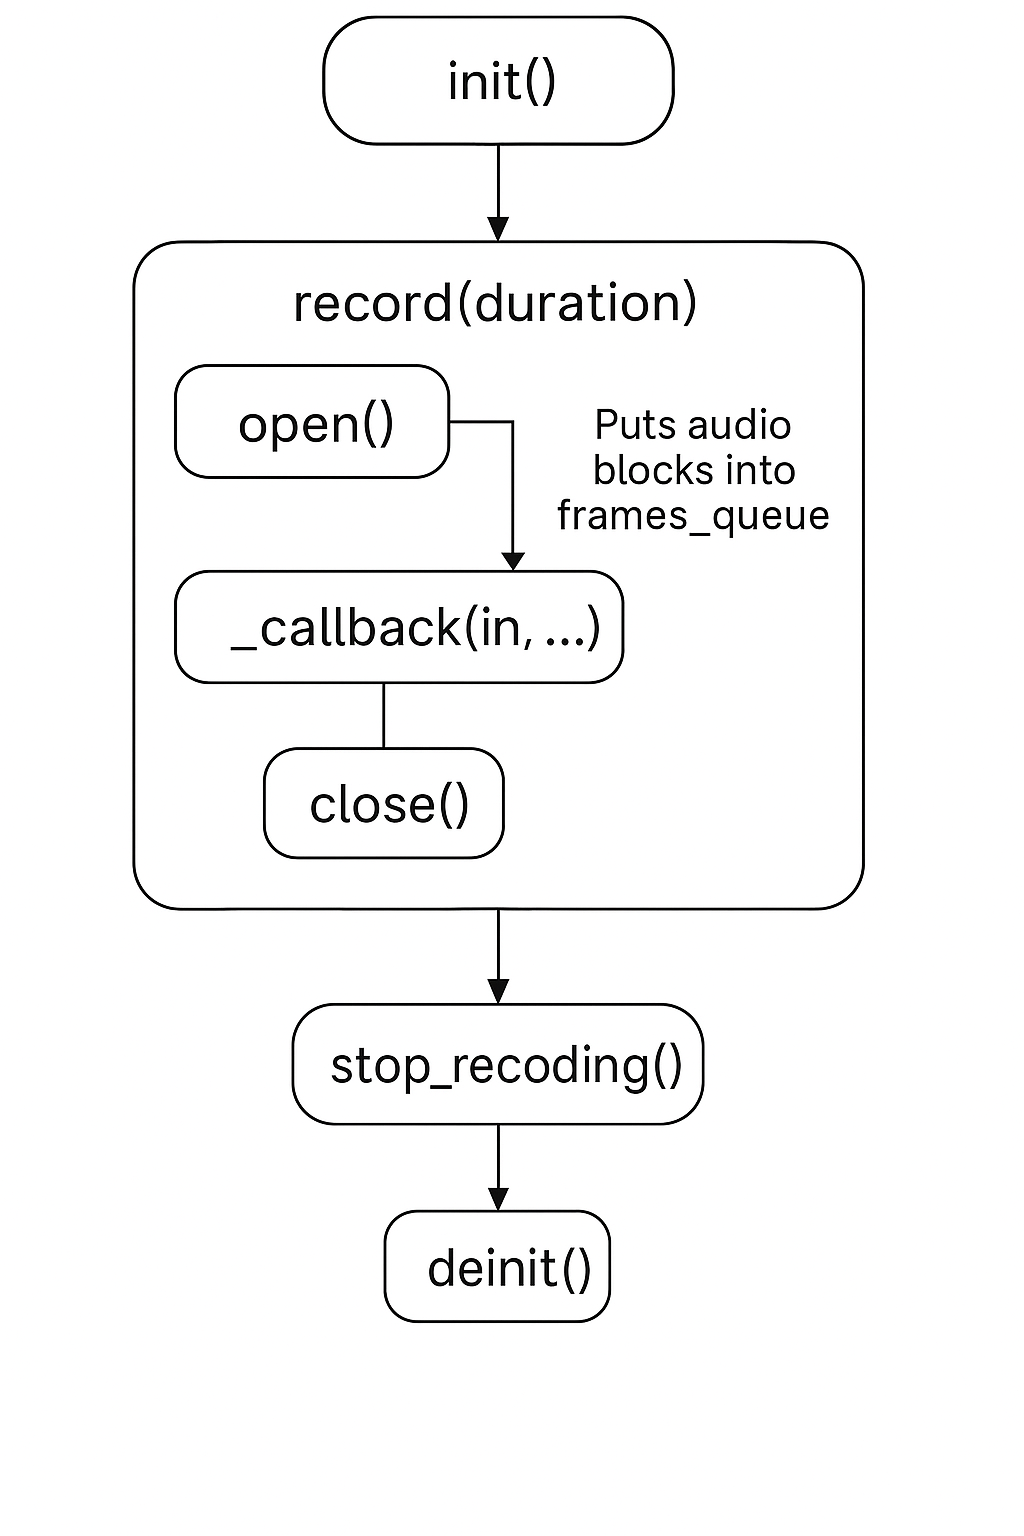
\includegraphics[width=0.6\textwidth]{graficos/workflow.png}
    \label{fig:workflow}
    \caption{Diagrama de flujo general de uso del módulo.}
\end{figure}




\subsection{Descripción de la clase y sus métodos}

\texttt{BehringerHandler} extiende de \texttt{BaseHandler} e implementa los métodos clave para el manejo del dispositivo. La utilización de una clase base común responde a una estrategia de diseño orientada a la modularidad y escalabilidad del sistema EAMRRA, donde múltiples módulos de adquisición o control comparten una estructura funcional similar. 

La clase \texttt{BaseHandler} actúa como plantilla abstracta, y define una interfaz mínima que obliga a los módulos derivados a implementar ciertos métodos esenciales, como \texttt{init}, \texttt{deinit}, \texttt{open} y \texttt{close}. Esta decisión asegura una simetría en la arquitectura del sistema, facilita el mantenimiento y permite la integración homogénea de nuevos módulos en el futuro. Además, permite aplicar patrones de programación como la inversión de dependencias, delegando a cada módulo el detalle de implementación mientras se conserva una estructura común y predecible.

A continuación se describen los métodos principales de la clase \texttt{BehringerHandler} con un detalle sobre los parámetros que reciben, los atributos que modifican, una descripción sintética de las acciones que realizan y finalmente, qué errores controlan, en cada caso.

\subsubsection*{Atributos principales definidos en \texttt{\_\_init\_\_}}

En el constructor se inicializan los siguientes atributos:

\begin{itemize}
    \item \texttt{audio\_interface}: objeto de PyAudio encargado de la comunicación con el hardware.
    \item \texttt{device\_index}: índice del dispositivo de audio identificado como Behringer.
    \item \texttt{stream}: flujo de entrada de audio (inicialmente \texttt{None}).
    \item \texttt{is\_recording}: bandera booleana que indica si una grabación está en curso.
    \item \texttt{recording\_thread}: hilo que ejecuta la escritura del audio en segundo plano.
    \item \texttt{start\_time}, \texttt{duration}: variables para controlar el tiempo de grabación.
    \item \texttt{frames\_queue}: cola de datos compartida entre el stream y el hilo de escritura.
    \item \texttt{logger}: objeto de \texttt{logging} configurado para registrar eventos en consola y archivo.
    \item \texttt{log\_file}, \texttt{output\_path}: rutas de archivo utilizadas durante la ejecución.
\end{itemize}

\subsubsection*{\texttt{init()}}

\begin{itemize}
    \item \textbf{Parámetros:} ninguno.
    \item \textbf{Atributos modificados:} \texttt{audio\_interface}, \texttt{device\_index}.
    \item \textbf{Acciones:} escanea los dispositivos de audio disponibles mediante \texttt{PyAudio} y selecciona automáticamente el que contiene ``Behringer'' o ``USB'' en su nombre, y tiene canales de entrada.
    \item \textbf{Control de errores:} si ya fue inicializado, emite un log y no repite el proceso. Si no encuentra el dispositivo, registra una advertencia. Si ocurre una excepción, se registra el error y se garantiza la liberación del objeto \texttt{PyAudio}.
\end{itemize}

\subsubsection*{\texttt{open()}}

\begin{itemize}
    \item \textbf{Parámetros:} ninguno.
    \item \textbf{Atributos modificados:} \texttt{stream}.
    \item \textbf{Acciones:} abre un flujo de entrada utilizando el índice del dispositivo detectado. Establece el formato en 24 bits, dos canales, 192 kHz y un tamaño de buffer de 8192 muestras.
    \item \textbf{Control de errores:} si el dispositivo no fue inicializado, se emite una advertencia. Si ocurre una excepción al abrir el flujo, se registra el error y el atributo \texttt{stream} se deja en \texttt{None}.
\end{itemize}

\subsubsection*{\texttt{record(duration)}}

\begin{itemize}
    \item \textbf{Parámetros:} \texttt{duration} (float), duración de la grabación en segundos.
    \item \textbf{Atributos modificados:} \texttt{is\_recording}, \texttt{start\_time}, \texttt{duration}, \texttt{recording\_thread}, \texttt{output\_path}.
    \item \textbf{Acciones:} crea el directorio \texttt{recordings} si no existe, genera un nombre de archivo único basado en fecha y hora, limpia la cola de audio, llama a \texttt{open()} y lanza un hilo que ejecuta \texttt{\_write\_audio()}.
    \item \textbf{Control de errores:} si el dispositivo no está inicializado, emite una advertencia y no comienza la grabación.
\end{itemize}

\subsubsection*{\texttt{\_write\_audio()}}

\begin{itemize}
    \item \textbf{Parámetros:} ninguno (método privado llamado por un hilo).
    \item \textbf{Atributos modificados:} ninguno directamente; opera sobre \texttt{frames\_queue}.
    \item \textbf{Acciones:} crea el archivo WAV, configura los parámetros del encabezado y escribe bloques de audio tomados desde \texttt{frames\_queue} hasta que finalice la grabación o la cola se vacíe.
    \item \textbf{Control de errores:} utiliza tiempo de espera en la cola para evitar bloqueos, registra la finalización y llama a \texttt{close()} al terminar.
\end{itemize}

\subsubsection*{\texttt{stop\_recording()}}

\begin{itemize}
    \item \textbf{Parámetros:} ninguno.
    \item \textbf{Atributos modificados:} \texttt{is\_recording}, \texttt{recording\_thread}.
    \item \textbf{Acciones:} cambia el estado de grabación, espera a que el hilo finalice (join) y limpia referencias.
    \item \textbf{Control de errores:} verifica que el hilo exista y esté activo antes de intentar finalizarlo. Registra eventos relevantes.
\end{itemize}

\subsubsection*{\texttt{close()}}

\begin{itemize}
    \item \textbf{Parámetros:} ninguno.
    \item \textbf{Atributos modificados:} \texttt{stream}.
    \item \textbf{Acciones:} detiene y cierra el flujo de audio si está activo, y libera la referencia.
    \item \textbf{Control de errores:} si no hay stream activo, emite una advertencia; si ocurre una excepción, se registra.
\end{itemize}

\subsubsection*{\texttt{deinit()}}

\begin{itemize}
    \item \textbf{Parámetros:} ninguno.
    \item \textbf{Atributos modificados:} \texttt{audio\_interface}, \texttt{device\_index}.
    \item \textbf{Acciones:} cierra el objeto \texttt{PyAudio} y limpia los atributos relacionados al dispositivo.
    \item \textbf{Control de errores:} si ya está desinicializado, se registra y se evita repetir el proceso.
\end{itemize}





\clearpage
\section{PRUEBAS Y ENSAYOS}

Para validar el correcto funcionamiento del módulo \texttt{BehringerHandler}, se desarrolló una batería de pruebas unitarias y funcionales empleando los marcos de prueba \texttt{unittest} y \texttt{pytest}, junto con técnicas de \textit{mocking} a través de \texttt{unittest.mock}. El objetivo principal de los ensayos fue asegurar la correcta inicialización del dispositivo, la grabación de audio, el manejo de errores y la robustez del sistema ante condiciones adversas.

El framework \texttt{unittest} forma parte de la biblioteca estándar de Python. Este framework sigue el modelo xUnit, ampliamente adoptado en distintos lenguajes de programación. Las pruebas se organizan en clases que heredan de \texttt{unittest.TestCase}. Cada método representa un caso de prueba individual. El framework proporciona métodos de aserción para validar el comportamiento del código bajo prueba. También permite configurar y limpiar el entorno de prueba mediante los métodos \texttt{setUp()} y \texttt{tearDown()}. En este proyecto, \texttt{unittest} sirvió como base para estructurar los casos que evalúan la inicialización del dispositivo, la grabación de audio, el manejo de errores y los mecanismos de cierre.

El framework \texttt{pytest} es una herramienta externa que amplía las capacidades de prueba en Python. Su sintaxis es más concisa y flexible que la de \texttt{unittest}. Las pruebas se pueden definir como funciones independientes, sin necesidad de clases. \texttt{pytest} también ofrece mecanismos potentes como las \textit{fixtures}, la captura de logs con \texttt{caplog} y una integración natural con \texttt{assert}. En este proyecto, \texttt{pytest} se utilizó para verificar el sistema de logging, simular errores y complementar los ensayos definidos con \texttt{unittest}.

Ambos frameworks resultan compatibles y pueden coexistir dentro del mismo entorno de pruebas. \texttt{unittest} aportó una estructura clásica y controlada para los casos más detallados. Por su parte, \texttt{pytest} ofreció herramientas modernas que facilitaron la validación de condiciones específicas, como el registro de advertencias y errores.

En el contexto de pruebas de software, un \textit{mock} es un objeto simulado. Este objeto reemplaza a una dependencia real y permite controlar su comportamiento durante los ensayos. El uso de \textit{mocks} facilita el aislamiento del componente que se desea evaluar. También permite verificar respuestas específicas ante distintos estímulos. En los ensayos del módulo \texttt{BehringerHandler}, se reemplazaron objetos como \texttt{pyaudio.PyAudio}, \texttt{wave.open}, \texttt{datetime.datetime} y \texttt{time.time}. Esta técnica hizo posible simular la presencia de dispositivos de audio. También permitió interceptar la creación de archivos sin escribir en el disco. Además, facilitó la generación de marcas de tiempo controladas y la simulación de condiciones temporales específicas. Gracias a este enfoque, se pudieron reproducir distintos escenarios. Por ejemplo, se evaluaron fallas de inicialización, errores de grabación y ausencia de datos en la cola, sin necesidad de depender de hardware real.

En los ensayos del módulo \texttt{BehringerHandler}, se utilizó una \textit{fixture} para reiniciar los manejadores del sistema de logging antes de cada prueba.  Una \textit{fixture} es una función o recurso que prepara el entorno antes de ejecutar una prueba. También puede encargarse de restaurar el estado original una vez finalizada la ejecución. En el marco de \texttt{pytest}, las \textit{fixtures} permiten definir comportamientos repetitivos de forma declarativa y reutilizable.  Esta estrategia evitó interferencias entre casos de prueba consecutivos. También permitió verificar con precisión los mensajes generados por el sistema, en combinación con la herramienta \texttt{caplog}.

\subsection{Cobertura de pruebas}

Las pruebas se estructuraron para cubrir los siguientes aspectos del módulo:

\begin{itemize} \item Inicialización del dispositivo de audio Behringer. \item Manejo de errores cuando el dispositivo no está disponible o es inválido. \item Grabación de audio y generación del archivo de salida en formato \texttt{.wav}. \item Validación del flujo de ejecución en presencia o ausencia de datos en la cola de audio. \item Verificación del correcto registro de mensajes en el sistema de logging. \item Evaluación del comportamiento de los métodos auxiliares, como \texttt{open()}, \texttt{close()} y \texttt{deinit()}. \end{itemize}

\subsection{Estrategia de prueba}

Se utilizaron técnicas de simulación (\textit{mocking}) para reemplazar el comportamiento del hardware de audio y del sistema de archivos, permitiendo un entorno controlado para la validación lógica del código. Particularmente, se realizaron los siguientes reemplazos:

\begin{itemize} \item \texttt{pyaudio.PyAudio}: Simulado para emular la presencia (o ausencia) del dispositivo Behringer. \item \texttt{wave.open}: Interceptado para evitar la creación real de archivos de audio. \item \texttt{datetime.datetime.now()}: Reemplazado para asegurar consistencia en los nombres de archivo generados. \item \texttt{time.time()}: Controlado para validar condiciones temporales durante la grabación. \end{itemize}

La ejecución de los ensayos se realiza desde la línea de comandos. Para ello, se utiliza el ejecutable de \texttt{pytest}, que detecta automáticamente todos los archivos de prueba cuyo nombre comienza con \texttt{test\_} o termina en \texttt{\_test.py}. El comando que se utiliza en el módulo \texttt{BehringerHandler} para lanzar todas las pruebas, que incluyen tanto las escrdefinidas para elitas con \texttt{unittest} como las específicas de \texttt{pytest}, es:

\begin{lstlisting}[language={python}]
pytest tests/modules/behringer/test_behringer_handler.py -v 
\end{lstlisting}



El modificador \texttt{-v} activa el modo detallado (\textit{verbose}), que muestra el nombre de cada prueba y su resultado. La salida por consola incluye también los logs generados durante la ejecución, lo que permite verificar que los mensajes esperados fueron correctamente emitidos.

\subsection{Casos de prueba destacados}

\begin{itemize} \item \textbf{Inicialización exitosa}: Se verifica que el dispositivo Behringer es detectado y que se almacena correctamente el índice del dispositivo. \item \textbf{Inicialización fallida}: Se simula la ausencia de dispositivos y se valida que el índice del dispositivo permanece \texttt{None}. \item \textbf{Grabación de audio}: Se simula una sesión de grabación, incluyendo escritura de datos en la cola, y se verifica la creación lógica del archivo de salida. \item \textbf{Manejo de cola vacía}: Se evalúa la robustez del sistema ante la ausencia de datos durante la grabación (control de excepciones por \texttt{queue.Empty}). \item \textbf{Log de advertencias}: Se valida que se emiten advertencias apropiadas cuando se intenta abrir o grabar sin haber inicializado el sistema. \item \textbf{Callback del flujo de audio}: Se prueba el comportamiento del método de \texttt{callback} tanto en estado de grabación como en reposo. \item \textbf{Cierre con errores}: Se simula una excepción al intentar cerrar un flujo de audio defectuoso y se verifica que se registre el error correspondiente. \end{itemize}

\subsection{Integración con Pytest}

Además de los tests basados en \texttt{unittest}, se incorporaron pruebas con \texttt{pytest} utilizando \texttt{fixtures} para configurar adecuadamente los manejadores de logging. Se utilizó \texttt{caplog} para capturar mensajes de log y confirmar que los errores y advertencias se registran correctamente.

\section{RESULTADOS}

Todas las pruebas fueron ejecutadas de forma automatizada y arrojaron resultados satisfactorios. No se detectaron fallos ni excepciones no controladas. El módulo demostró comportarse de forma robusta frente a condiciones esperadas y adversas, lo cual valida su uso en entornos complejos de adquisición de señales de audio para aplicaciones tanto de laboratorio como de campo.

En la figura \ref{fig:testUni} se pueden observar los resultados obtenidos al ejecutar veinte pruebas unitarias al código.  Se puede apreciar que todas las pruebas fueron exitosas. 

\begin{figure}[htpb]
    \centering
    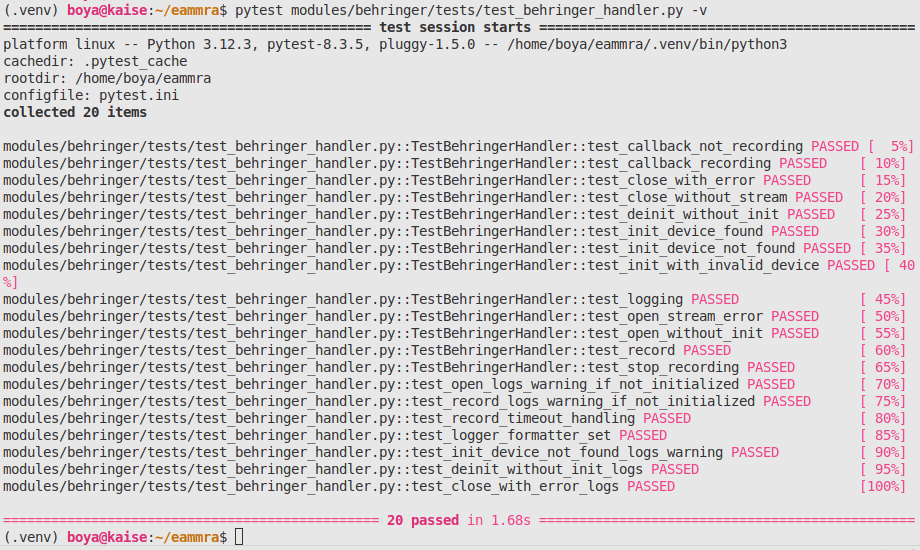
\includegraphics[width=\textwidth]{graficos/unittest.png}
    \caption{Resultados de test unitarios al código.}
    \label{fig:testUni}
\end{figure}

Un test de cobertura permite medir qué proporción del código fuente es ejecutada durante la realización de las pruebas. Esta métrica es útil para identificar partes del código que no fueron evaluadas y, por lo tanto, podrían contener errores no detectados. Para calcular la cobertura en este proyecto, se utilizó el plugin \texttt{pytest-cov}, que extiende \texttt{pytest} con opciones específicas. La cobertura se aplicó al módulo \texttt{behringer\_handler.py} y se ejecutó con el siguiente comando:

\begin{lstlisting}[language=bash] 
pytest --cov=modules.behringer.behringer_handler modules/behringer/tests/
 --cov-report=term-missing -v 
\end{lstlisting}

La salida del análisis mostró una cobertura del 96\%. De un total de 129 líneas ejecutables, 5 no fueron alcanzadas por las pruebas. Las líneas omitidas se encuentran en las posiciones 49–50, 72–73 y 101 del archivo fuente. Esta información resulta valiosa para planificar nuevas pruebas que completen la validación del módulo.

\begin{figure}[htpb]
    \centering
    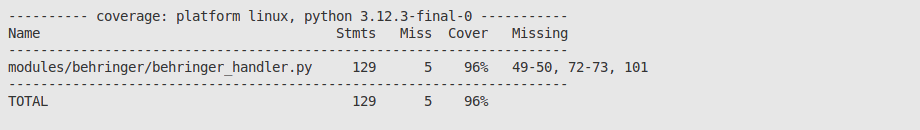
\includegraphics[width=\textwidth]{graficos/coverage.png}
    \caption{Ejecución de pruebas con medición de cobertura.}
    \label{fig:testCov}
\end{figure}


\clearpage
\section{CONCLUSIONES}

El desarrollo del módulo \texttt{BehringerHandler} permitió incorporar una solución robusta y extensible para la configuración y el control de la interfaz de audio Behringer UMC204HD en el sistema EAMMRA. Su diseño modular y su implementación en Python favorecen la integración con otros componentes del sistema y facilitan el mantenimiento y la evolución futura del software.

Durante el proceso de desarrollo, se aplicaron buenas prácticas de codificación basadas en las guías PEP-8 y PEP-257. Se emplearon herramientas de análisis estático como Flake8, Pylint y Black, que contribuyeron a mejorar la legibilidad, la coherencia y la calidad general del código. Estas herramientas resultaron fundamentales para reducir defectos y facilitar el trabajo colaborativo en el proyecto.

La validación funcional del módulo se realizó mediante una batería de pruebas automatizadas. Se utilizaron los marcos \texttt{unittest} y \texttt{pytest}, junto con técnicas de \textit{mocking} y \textit{fixtures}, que permitieron verificar el comportamiento del sistema bajo distintas condiciones, sin necesidad de depender del hardware real. Las pruebas contemplaron tanto situaciones normales como escenarios de falla y manejo de errores.

Los resultados de las pruebas indicaron un funcionamiento correcto y estable del módulo. No se detectaron errores durante la ejecución, y la cobertura alcanzó el 96\% de las líneas ejecutables. Este nivel de cobertura refleja un alto grado de confianza en el comportamiento del módulo ante condiciones esperadas y adversas.

Como línea futura de trabajo, se propone implementar pruebas de integración en conjunto con otros módulos del sistema EAMMRA, así como ensayos funcionales en condiciones reales de operación. También se sugiere completar la cobertura restante, documentar formalmente la API del módulo, y evaluar mecanismos de tolerancia a fallos para mejorar su desempeño en entornos hostiles o de difícil acceso.
%

% =====================================================================================================
% =====================================================================================================
% PÁGINA DE REFERENCIAS
% =====================================================================================================
% =====================================================================================================

\clearpage

\addcontentsline{toc}{section}{REFERENCIAS}
\bibliographystyle{apa-good}	% (uses file "plain.bst")
\bibliography{7_Referencias}	% Acá está la base de datos de referencias. Espera el archivo "7_Referencias.bib"

\clearpage

% =====================================================================================================
% =====================================================================================================
% APÉNDICE
% =====================================================================================================
% =====================================================================================================

%
%% Reseteo y cambio de numeración para los apéndices
%\setcounter{section}{0}
%\renewcommand\appendix{\Roman{section}}
%%\def\thesection{\Roman{section}}
%
%\appendix
\appendixpage
\addappheadtotoc
\section{Desarrollo de códigos en MATLAB para visualización de esferoides prolados y oblados.}
\label{pendiceA}
Un esferoide prolado $E\subset R^3$  puede quedar descripto por dos parámetros. Éstos pueden ser: 
Los Semiejes mayor y menor, $a$ y $b$, siendo a la máxima distancia desde el origen de coordenadas sobre
el eje $x$, y $b$ la máxima distancia desde el origen sobre el eje $z$. 
\[
\frac{x^2}{a^2} + \frac{y^2}{a^2} + \frac{z^2}{b^2} =1
\]



% Viejo método de apéndice es poner un comando \appendix antes del include correspondiente a este archivo para luego en el archivo '8_Apendices.tex' tipear cada sección del apéndice así:
%
%		\addcontentsline{toc}{section}{APÉNDICE I}
%		\section*{APÉNDICE I}
%		\subsection*{{Desarrollo de códigos en MATLAB para visualización de esferoides prolados y oblados.}
%		\label{pendiceA}

%

\end{document}

